% TITLE:
% Author: Adrian Schrader
% Created on: 31/7/15

\documentclass[a4paper, 10pt, twocolumn]{scrartcl}
\usepackage[ngerman]{babel}

% Mathematics
\usepackage{amsmath}
\usepackage{amssymb}
\numberwithin{equation}{subsection}

% Font and Style
\usepackage{ucs}
\usepackage[T1]{fontenc}
\usepackage{abstract}
\usepackage{url}
\usepackage{lipsum}
\usepackage{hyperref}
\hypersetup{colorlinks=false}

% Font Package (select one)
%\usepackage{lmodern}
%\usepackage{kpfonts}
%\usepackage{ccfonts}
%\usepackage[light]{cmbright}
%\usepackage{antpolt}
\usepackage[light]{iwona}

% Bibliography
\usepackage[numbers,round]{natbib}
\usepackage[babel,german=guillemets]{csquotes}
\bibliographystyle{alphadin}

% Image and Graphics
\usepackage{graphicx}
\usepackage{dblfloatfix}
\usepackage[left=2.5cm, right=2.5cm, top=2.5cm, bottom=4.5cm]{geometry}
\setlength{\columnsep}{15pt}

% Document Information
\title{Fouriertransformation}
\subtitle{Hintergrund, Beispiele und Anwendungen von Frequenzanalysen}
\author{Adrian Schrader}
%\subject{Schriftliche Ausarbeitung, Physik, Kuhn}
\date{\today}

\begin{document}
  % Create Title, Abstract and TOC
  \twocolumn[\maketitle \begin{abstract} \begin{minipage}{1.0\linewidth}
  % Abstract: Zusammenfassung des Inhalts
In allen Wissenschaftsfeldern ist die Interferenz von Signalen ein Problem für Analytik und Verarbeitung. Die Fourieranalyse und ihre Varianten bilden bis heute ein mächtiges Werkzeug, um zeitabhängige Signale in ihr Frequenzsprektrum aufzuspalten und zu analysieren. Dieses Paper bietet ausführlichere Beschreibungen zu den Beispielen und mathematische Hintergründe zum Vortrag \glqq Fourieranalyse - Hintergründe und Anwendungen von Frequenzanalysen\grqq.

  \vspace{0.8cm}
  \end{minipage}\end{abstract} ]

  \tableofcontents

  % CONTENT
  % MATHEMATISCHER HINTERGRUND UND HERLEITUNG

\section{Mathematische Herleitung}

\subsection{Hintergrund}
Eine Hauptcharakteristik aller Wellen ist ihre gegenseitige Interferenz. Verschiedene Frequenzen, die sich im gleichen Medium befinden, können sich überlagern und sich so zu komplexen Signalen zusammenfügen. Mathematisch wird die Interferenz durch die Summe zweier Funktionen beschrieben.

\begin{align}
  s_{ges}(t) &= s_1(t) + s_2(t) + s_3(t) + ...
           %&= \hat{s}_1 \cdot sin(\omega_1 \cdot t + \phi_1)\\
           %&+ \hat{s}_2 \cdot sin(\omega_2 \cdot t + \phi_2)\\
           %&+ \hat{s}_3 \cdot sin(\omega_3 \cdot t + \phi_3)
\end{align}

Der französische Mathematiker und Physiker Jean Baptiste Joseph Fourier postulierte Anfang des 19. Jahrhunderts, dass sich alle Funktionen als Summe von Grund- und Oberschwingungen ausdrücken lassen sollten und entwarf eine Methode, die Amplituden der einzelnen Frequenzen zu berechnen.

Erst Peter Gustav Lejeune Dirichlet und Bernhard Riemann formulieren Fouriers Vermutung konkret und konnten beweisen, dass seine trigonometrischen Reihen tatsächlich zur ursprünglichen Funktion konvergieren \cite{art:konyagin00}.

\begin{align}
  f_N(x) &= \sum_{n=-N}^{N} \hat{f}(x) e^{i n x} \\
  f(x) &\overset{?}{=}\lim_{N \to \infty}{f_N(x)}
\end{align}

\subsection{Fourierreihe}
Aus der Annahme, dass alle Funktionen als Summe von trigonometrischen Funktionen darstellbar sind, lässt sich eine allgemeine Darstellungsweise als Grundlage für die Herleitung aufstellen.
Die in Gleichung \ref{algn:fourier_sums} dargestellten Formen enthalten alle eine Möglichkeit der Phasenverschiebung untereinander durch Einbinden des Phasenwinkels $ \varphi_n $ oder durch die gegeneinander verschobenen Sinus- und Kosinusfunktionen. Hierdurch entstehen je zwei neue, von der Kreisfrequenz abhängige, Variablen. In \ref{algn:fourier_sums_complex} werden die Sinus- und Kosinusfunktionen durch die eulersche Formel $ e^{i \theta} = cos(\theta) + i \cdot sin(\theta) $ zusammengefasst.

\begin{align}
  f(x) &= \sum_{n = 0}^{\infty} A_n cos(n x + \varphi_n)  \notag\\
  &= \frac{a_0}{2} + \sum_{n = 1}^{\infty} a_n cos(n x) + \sum_{n = 1}^{\infty} b_n sin(n x) \label{algn:fourier_sums} \\
  f(x) &= \sum_{n = 0}^{\infty} \alpha_n e^{i n x} \label{algn:fourier_sums_complex}
\end{align}

Durch Ermitteln dieser amplitudenbeschreibenden Variable $\alpha_n$ lässt sich die Funktion mit der so genannten \emph{Fourier-Synthese} neu zusammensetzen. Sie muss also den gleichen Informationsgehalt wie die Ursprungsfunktion $f(x)$ haben. Deshalb können wir Sie als Ergebnis der Transformation definieren.

\begin{align}
  f(t) &= \sum_{\omega = 0}^{\infty} \hat{f}(\omega) e^{i \omega t} \notag \\
  \mathcal{F}(f)(\omega) &= \hat{f}(\omega) \label{algn:ftrans}
\end{align}

\subsection{Fourieranalyse}

Der mathematisch weniger relevante, für die Physik jedoch umso bedeutendere Teil von Fouriers Entdeckung ist das Aufspalten eines Signals in die Amplituden seiner Frequenzen. Diese Zerlegung in die Harmonischen nennt sich \emph{Fourieranalyse}.

\subsubsection*{Darstellung durch Hilberträume}
Damit wir tatsächlich jede Funktionen als Summe von Vielfache von $ sin(n x)$, $cos(n x)$ und $1$, also unseren Funktionsbasen, ausdrücken zu können, brauchen wir eine allgemeine Schreibweise.

\begin{align}
  f(x) &= \frac{a_0}{2} + \sum_{n = 1}^{\infty} a_n cos(n x) + \sum_{n = 1}^{\infty} b_n sin(n x) \label{algn:allgSinCos}
\end{align}

Nun wird nur noch ein Operator gesucht, der auf die ursprüngliche Funktion und die gewünschte Funktionsbasis angewendet den jeweiligen Vorfaktoren zurückgibt. Am Beispiel der Sinusfunktion könnte das so aussehen wie in \ref{algn:skalarprodukt}. Der erwartete Rückgabewert wäre in diesem Falle $b_n$.

\begin{align}
  \langle f(x), sin(n x) \rangle &= \langle \frac{a_0}{2}, sin(n x) \rangle \notag\\
  &+ \sum_{n = 1}^{\infty} a_n \langle cos(n x), sin(n x) \rangle \notag \\
  &+ \sum_{n = 1}^{\infty} b_n \langle sin(n x), sin(n x) \rangle \label{algn:skalarprodukt}
\end{align}

Damit als Lösung nur noch $b_n$ übrig bleibt, ergeben sich verschiedene Eigenschaften für den gewünschten Operator. Im Folgenden gilt $ \{ v, w, u \in \{ sin(n x), cos(n x), 1 \}\} $

\begin{enumerate}
  \item \textbf{Linearität} Jeder Summand muss einzeln erfasst und der erwünschte Koeffizent ausgeklammert werden können. Es muss also gelten: $\langle \alpha \cdot v + \beta \cdot w, u \rangle = \alpha \cdot \langle v, u \rangle + \beta \cdot \langle w, u \rangle $
  \item \textbf{Orthogonalität (Interfunktionell)} Damit die nicht relevanten Funktionsbasen ausgeblendet werden können, muss der Operator zwischen den  unterschiedlichen Funktionsbasen null ergeben. Es gilt: $ \langle v_i, u_j \rangle = 0 $
  \item \textbf{Orthogonalität (Intrafunktionell)} Der jeweilige Koeffizient gehört immer zu einer spezifischen Frequenz, die anderen Frequenzen sollen als Produkt null ergeben. Damit gilt die Orthogonalität für die gleiche Grundfunktion, wenn diese unterschiedliche Frequenzen darstellen: $ \langle v_i, v_j \rangle = 0 \, | \, i \not= j $
  \item \textbf{Normierung} Der Operator zwischen zwei identischen Funktionen soll immer 1 ergeben, damit nur noch der ausgeklammerte Vorfaktor übrig bleibt. Es gilt: $ \langle v_i, v_i \rangle = 1 \, | \, i = j $
\end{enumerate}

In der Sprache der Mathematik würde man sagen, dass hier ein Hilbertraum aufgestellt wurde, der aus dreidimensionalen Vektoren besteht. Das Skalarprodukt (wir nannten es Operator) definiert den Vektorraum, indem er die Orthonormalbasen (wir nannten sie Funktionsbasen) festlegt und normiert. Auch ein Hilbertraum nutzt die oben angeführten Vorrausetzungen. \cite{web:gsi98}

Durch die Symmetrieeigenschaften der Sinus und Kosinusfunktionen können wir versuchen ein Skalarprodukt mit genau diesen Eigenschaften zu finden.

\begin{align}
  sin(- k \cdot x) = - sin(k \cdot x) \\
  cos(- k \cdot x) = cos ( k \cdot x)
\end{align}

Die Mittelwertsfunktion über eine Periode ist das gesuchte Skalarprodukt. Der Flächeninhalt unter $sin(k x)$ und $cos(k x)$ beträgt in einer Periode null, der Flächeninhalt unter den Quadraten der Funktionen ergibt $\pi$.

\begin{align}
  \langle f, g \rangle = \frac{1}{\pi} \int_{-\pi}^{\pi} f(x) \cdot g(x) \, dx
\end{align}

Mit den eingesetzten Orthonormalbasen ergibt das Skalarprodukt die Transformation für die Fourierreihe. Der Orthonormalvektor $1$ lässt sich als Spezialfall der Kosinusfunktion mit $cos(0) = 1$ ausdrücken.

\begin{align}
  a_n = \frac{1}{\pi} \int_{-\pi}^{\pi} f(t) \cdot cos(n \cdot t) \, dx \notag\\
  b_n = \frac{1}{\pi} \int_{-\pi}^{\pi} f(t) \cdot sin(n \cdot t) \, dx
\end{align}

Mit den anderen allgemeinen Darstellungsformen kann ebenso vorgegangen werden. Auch die komplexe Schreibweise teilt die Symmetrie und Integraleigenschaften, wie die trigonometrischen Funktionen. Damit gilt für die periodische Fouriertransformation:

\begin{align}
  \mathcal{F}(f)(\omega) &= \hat{f}(\omega) = \frac{1}{2 \pi} \int_{-\pi}^{\pi} f(t) \cdot e^{-i \omega t} \, dt
\end{align}

  \section{Diagramme und Darstellungen}

\begin{frame}
  \frametitle{FFT und Frequenzspektren}
  \begin{figure}
    \centering
    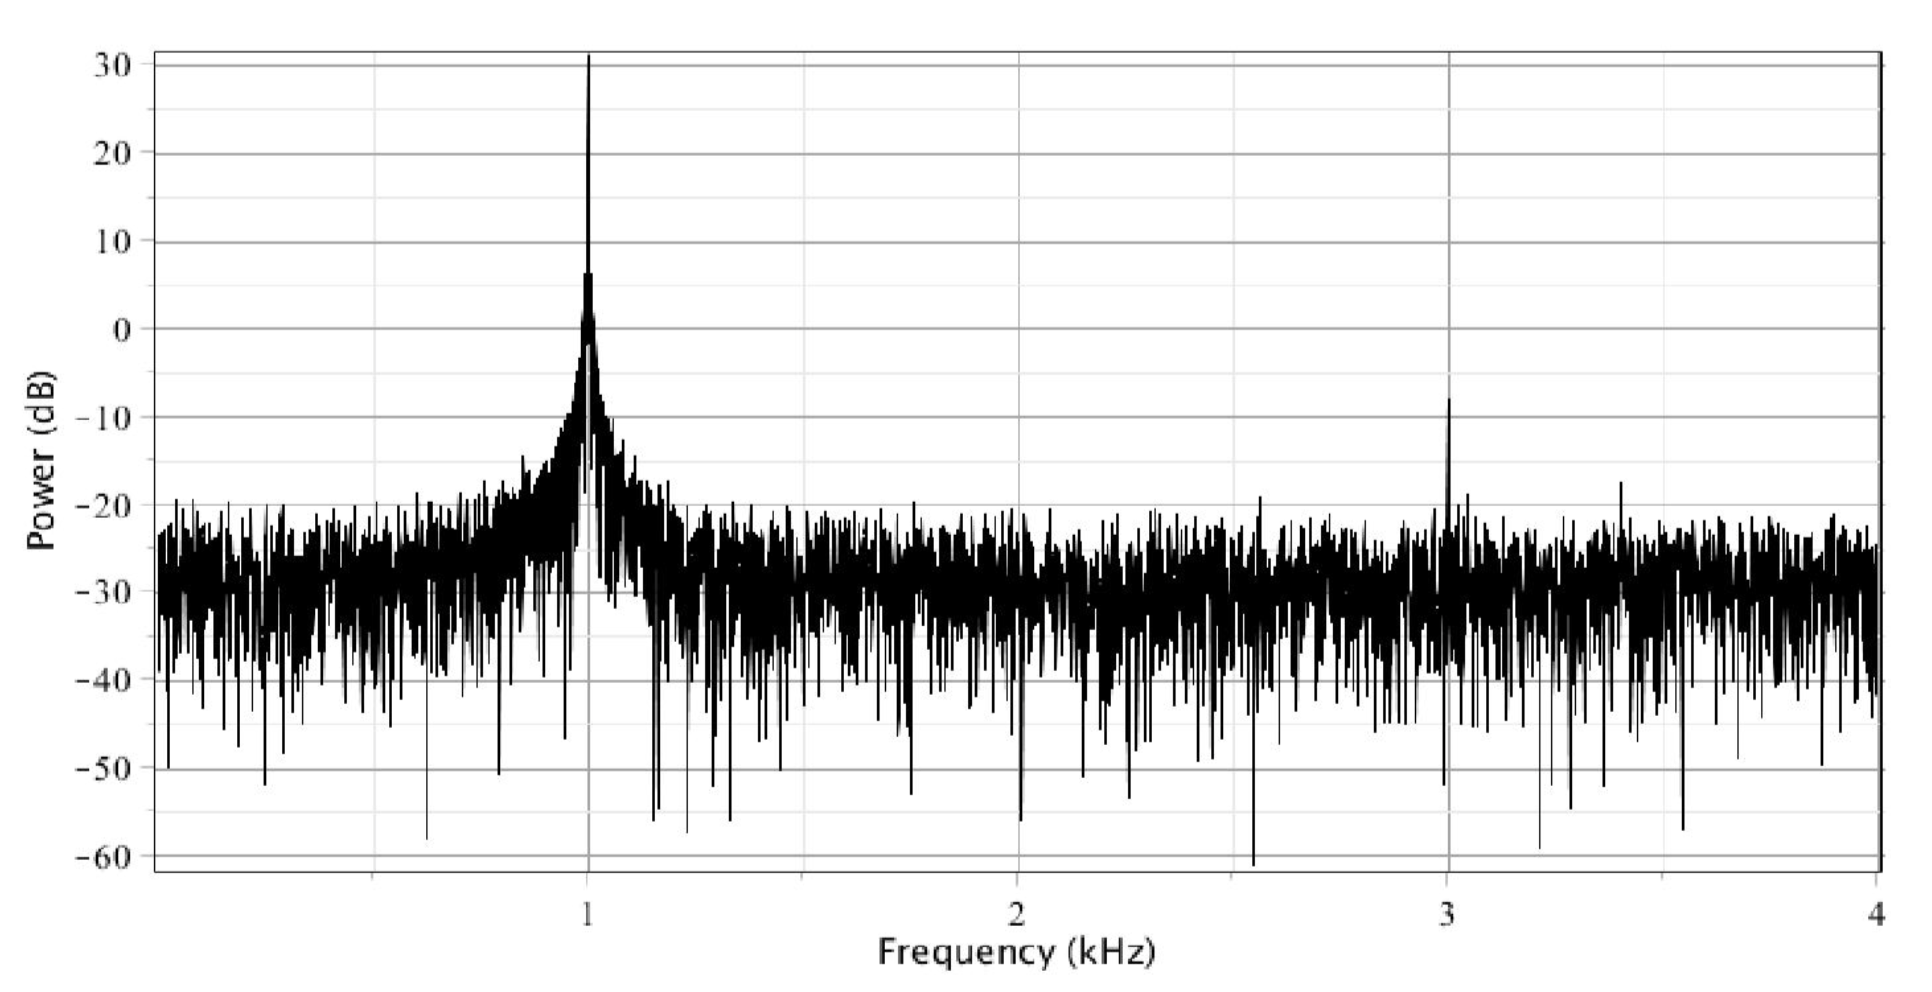
\includegraphics[width=\linewidth]{img/1khz_power}
    \caption{\url{ http://www.maplesoft.com/products/maple/features/Signal_Processing.aspx},  21.11.15}
  \end{figure}
\end{frame}

\begin{frame}
  \frametitle{Spektrogramme}
  \begin{figure}
    \centering
    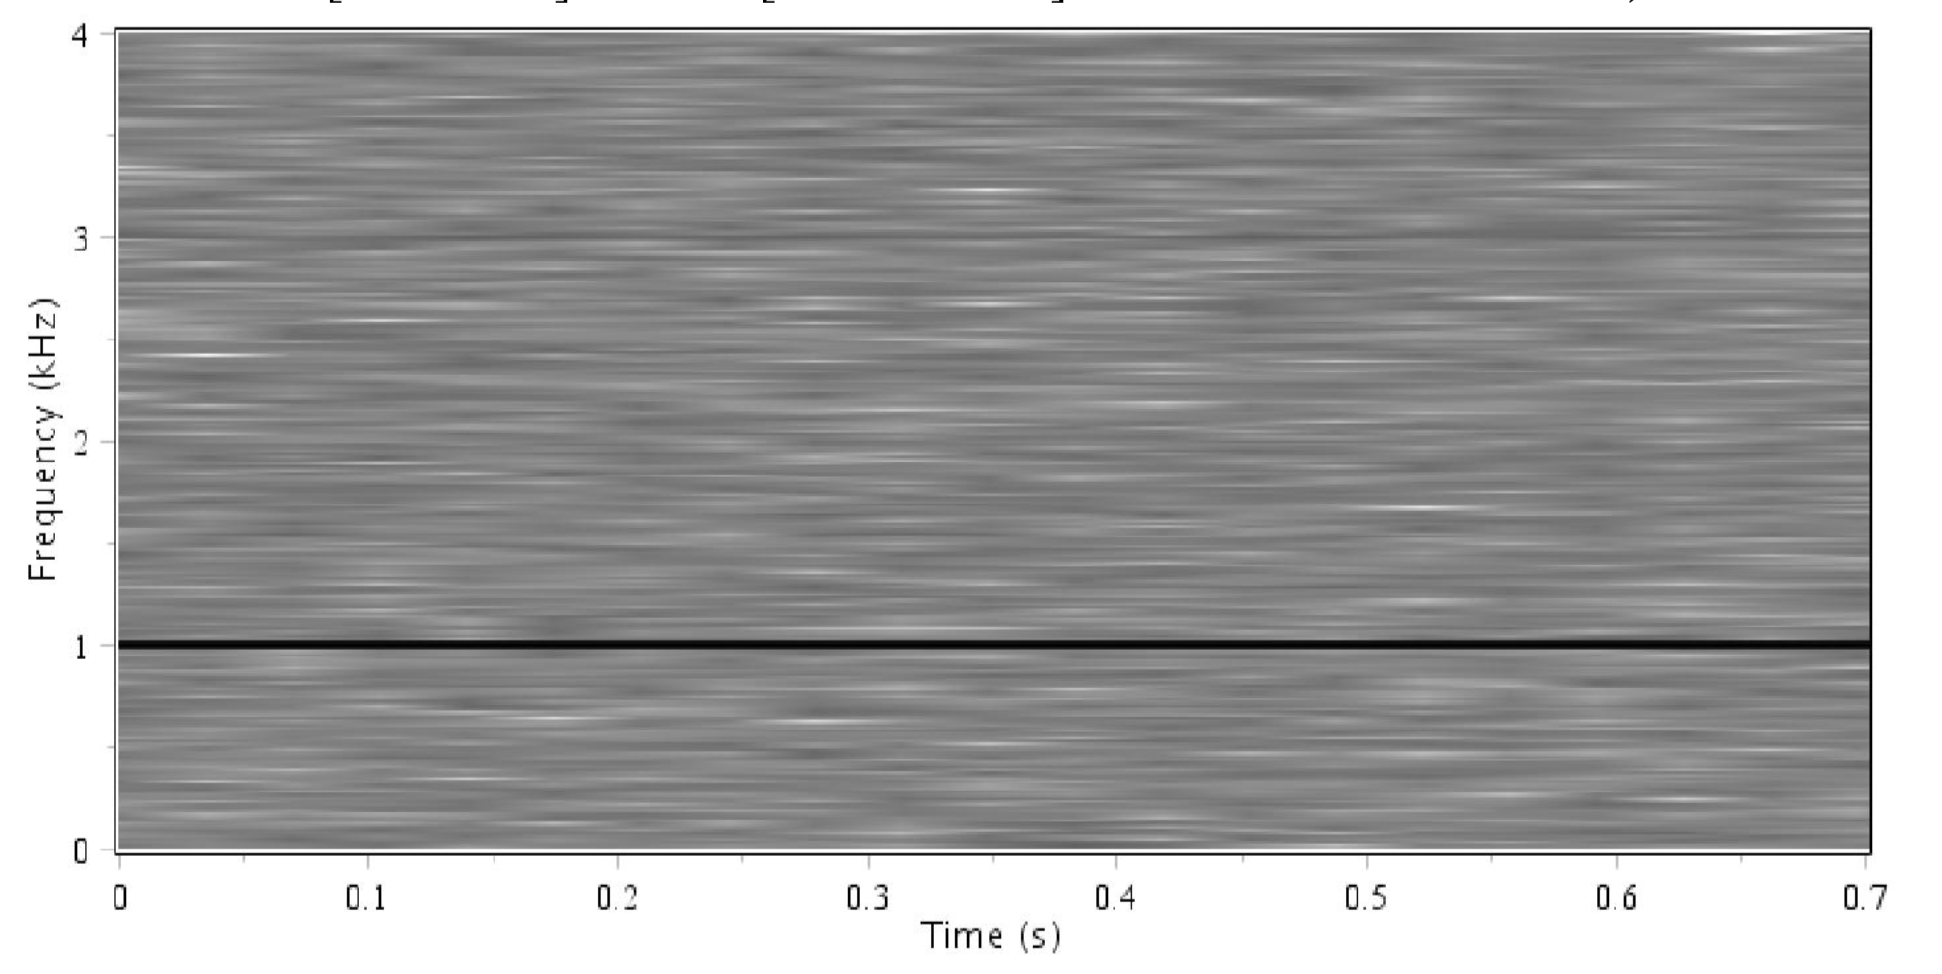
\includegraphics[width=\linewidth]{img/1khz}
    \caption{\url{ http://www.maplesoft.com/products/maple/features/Signal_Processing.aspx}, 21.11.15}
  \end{figure}
\end{frame}

  \section{Anwendungen und Beispiele}

\subsection{Klangwiedergange einer Geige}

\begin{frame}
  \frametitle{Klangcharakteristika einer Geige}
  \begin{figure}
    \centering
    \only<1>{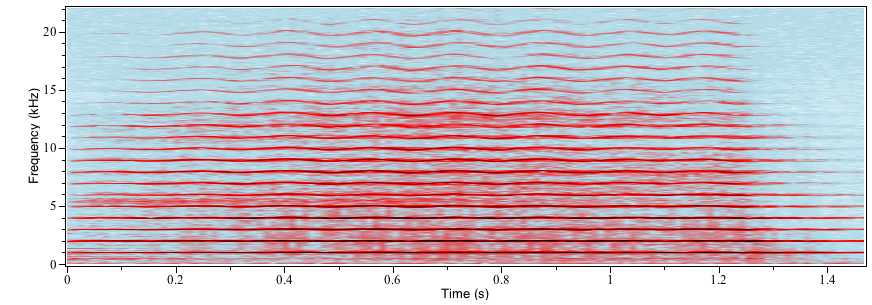
\includegraphics[width=\linewidth]{img/violin}}
    \only<2>{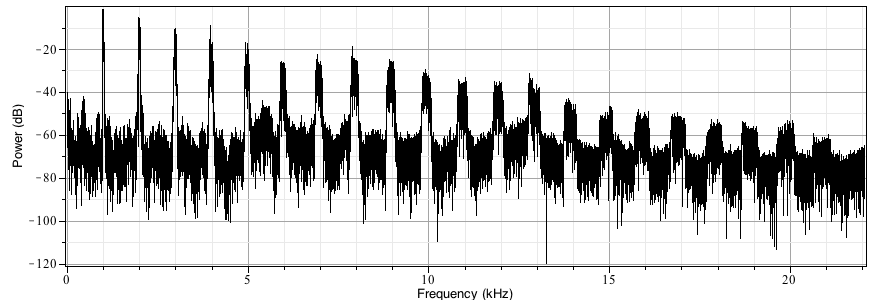
\includegraphics[width=\linewidth]{img/violin_power}}
    \label{img:violin}
  \end{figure}
\end{frame}

\subsection{Charakteristika von Sprache}

\begin{frame}
  \frametitle{Sprache}
    \begin{figure}
      \centering
      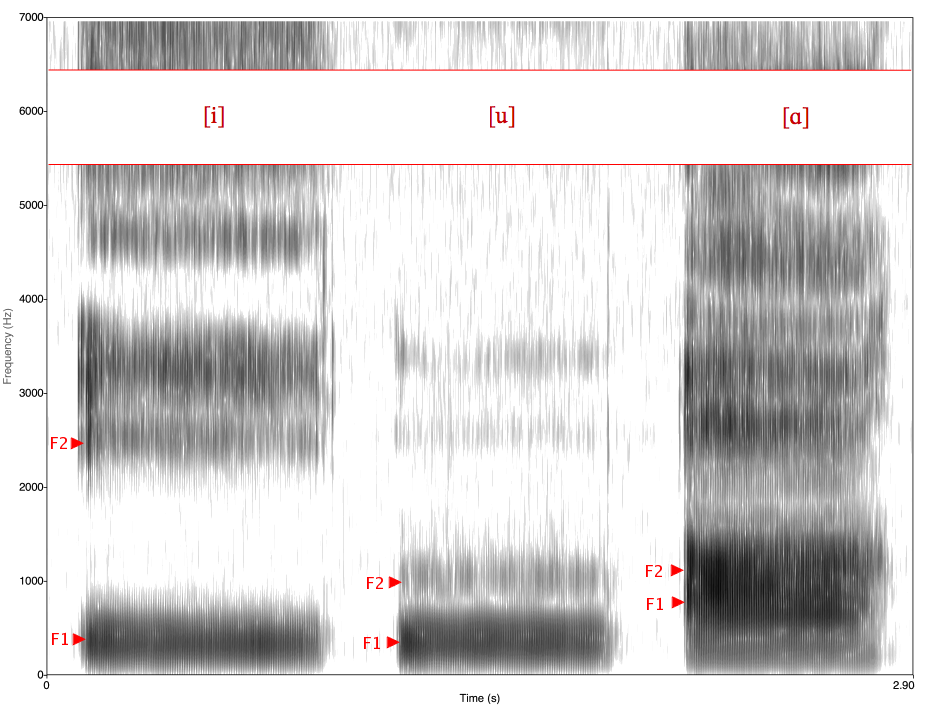
\includegraphics[width=0.8\linewidth]{img/iua}
      \label{img:vowls}
      \caption{\url{https://commons.wikimedia.org/wiki/File:Spectrogram_-iua-.png}, 02.12.15}
    \end{figure}
\end{frame}

\begin{frame}
  \frametitle{Sprache}
    \begin{figure}
      \centering
      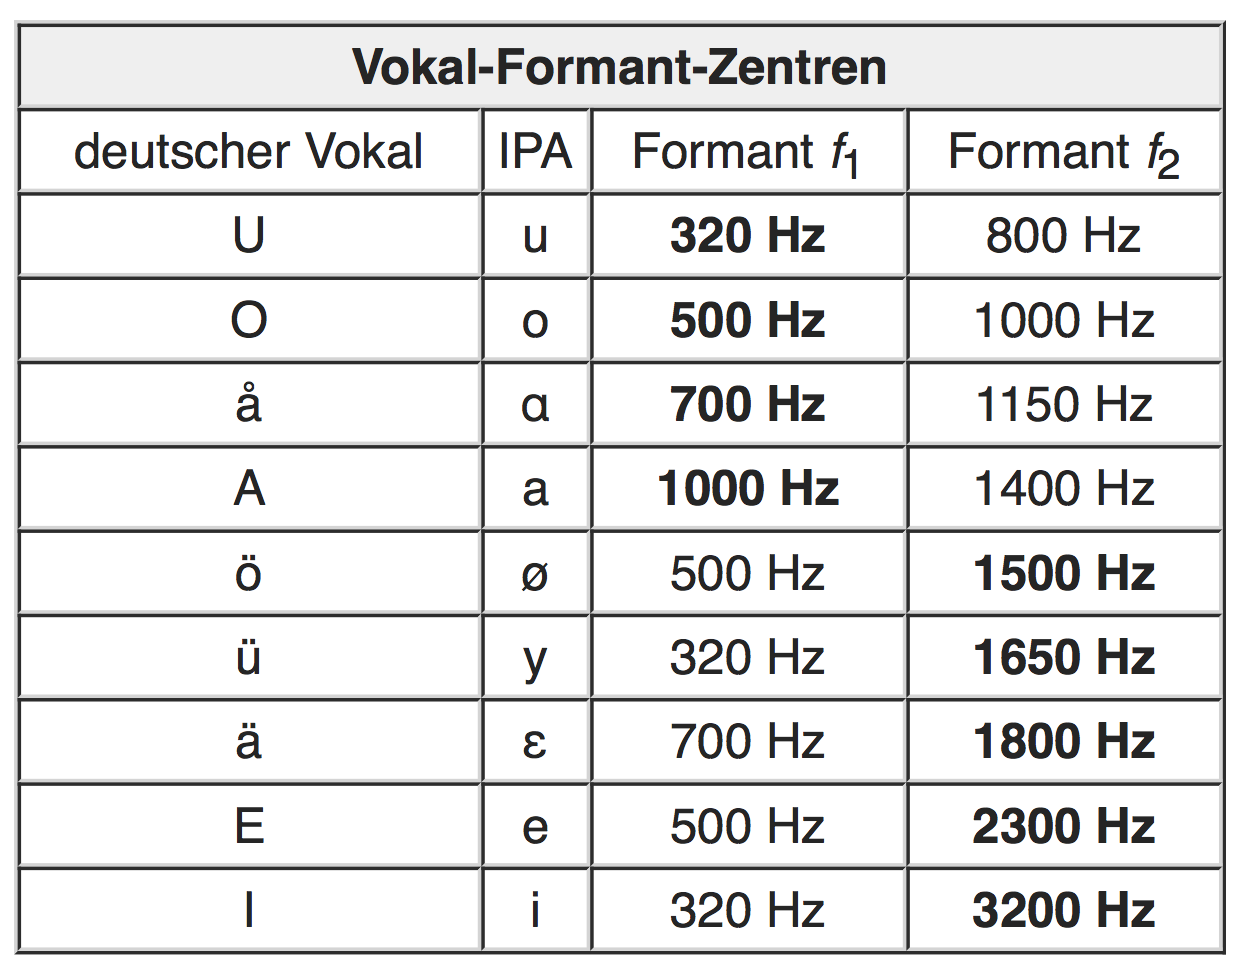
\includegraphics[width=0.8\linewidth]{img/formanten}
      \label{img:vowls}
    \end{figure}
\end{frame}


  % Bibliography
  \bibliography{bib/bibliography.bib}
\end{document}
